\documentclass[12pt,a4paper]{article}
\pdfoutput=1

%%
%% This huge block of usepackages does a lot of things.
%% It makes the text pritty on screens and ensures that you can use some common
%% tools.
%%

\usepackage[utf8]{inputenc}
\usepackage[T1]{fontenc}
% change language to whatever you write in
\usepackage[english]{babel}
\usepackage{amsmath}
\usepackage{lmodern}
\usepackage{listings}
\usepackage{units}
\usepackage{icomma}
\usepackage{color}
\usepackage{graphicx}
\usepackage{multicol,caption}
\usepackage{bbm}
\usepackage{hyperref}
\usepackage{xfrac}
\newcommand{\N}{\ensuremath{\mathbbm{N}}}
\newcommand{\Z}{\ensuremath{\mathbbm{Z}}}
\newcommand{\Q}{\ensuremath{\mathbbm{Q}}}
\newcommand{\R}{\ensuremath{\mathbbm{R}}}
\newcommand{\C}{\ensuremath{\mathbbm{C}}}
\newcommand{\rd}{\ensuremath{\mathrm{d}}}
\newcommand{\id}{\ensuremath{\,\rd}}

% This creates a nice figure environment that puts the image where you use it,
% and not where LaTeX wants it to be.
\newenvironment{Figure}
  {\par\medskip\noindent\minipage{\linewidth}}
  {\endminipage\par\medskip}

% neat horisontal line
\newcommand{\HRule}{\rule{\linewidth}{0.5mm}}

\begin{document}

\title{TNM087 – Colorizing the Prokudin-Gorskii Collection}
\author{Klas Eskilson (klaes950)}
\date{\today}

%%
%% Use one of these title methods
%%
\maketitle % simple latex title

\pagenumbering{arabic} % Arabic page numbers (and reset to 1)

\begin{Figure}
  \centering
    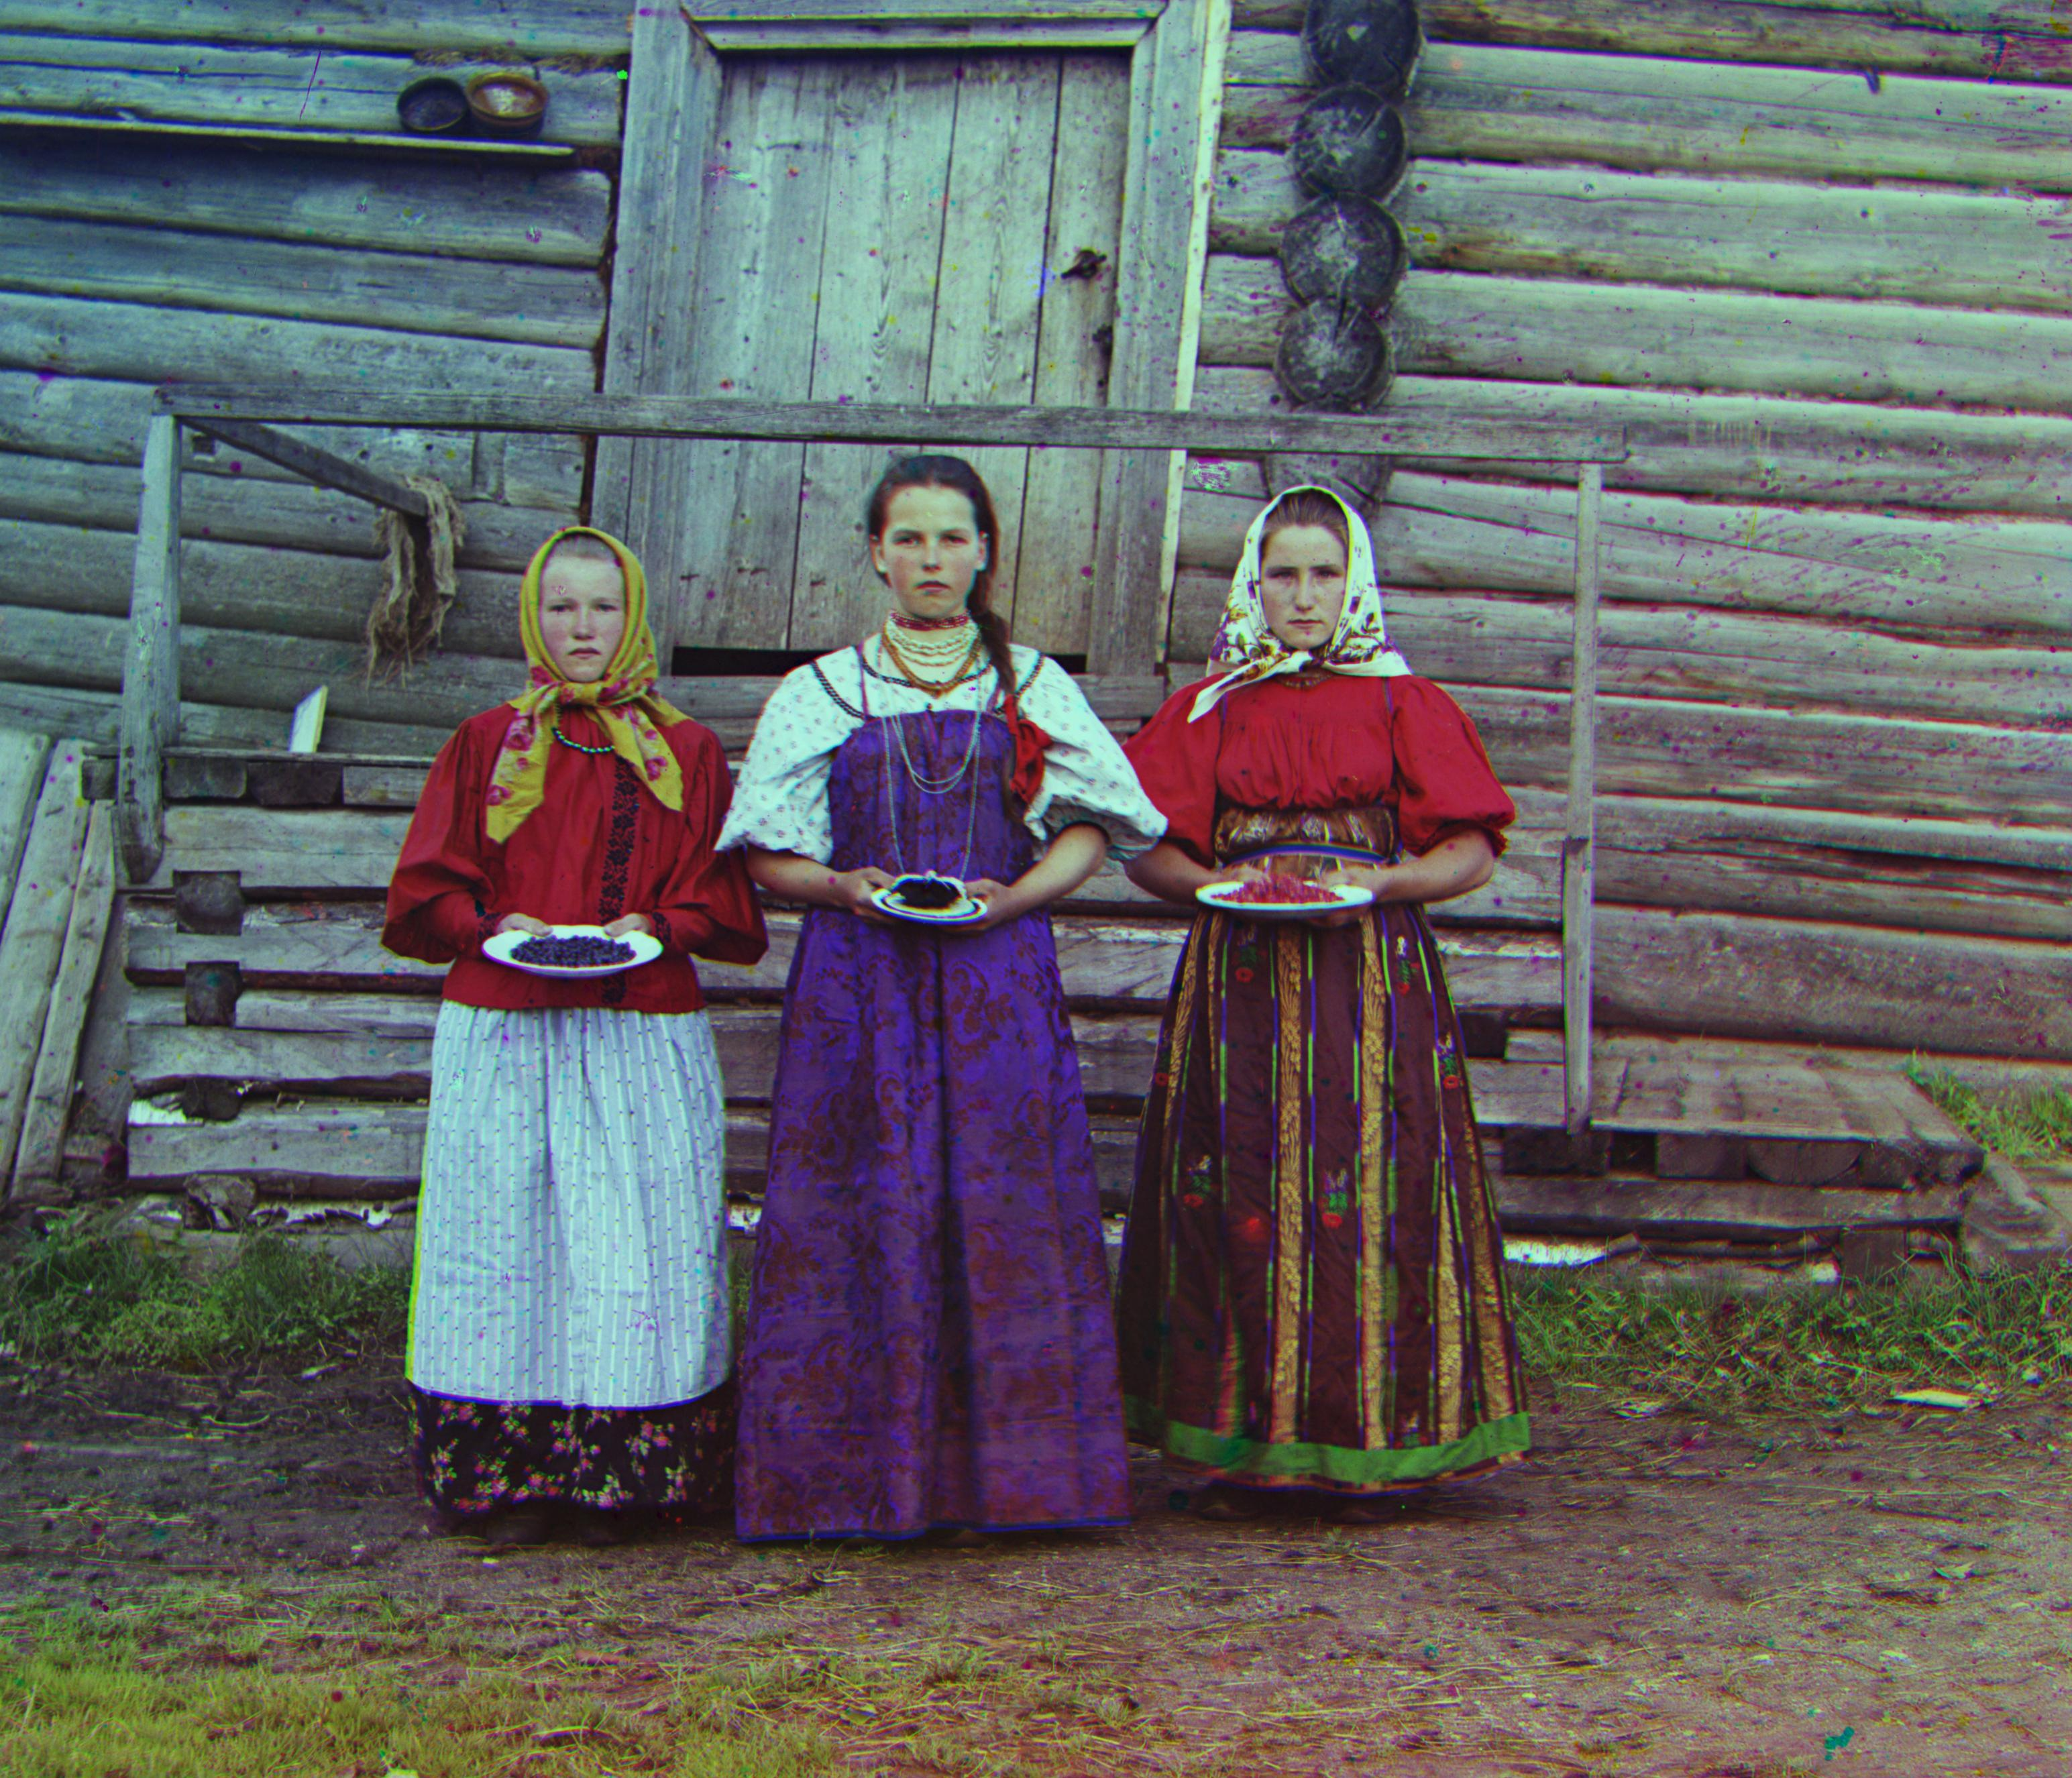
\includegraphics[width=0.8\textwidth]{result.jpg}
    \captionof{figure}{Final result.}
    \label{fig:final_result}
\end{Figure}

\section*{Introduction}

  This report covers lab 4 of the Image processing and analysis course and the issue of colorizing the Prokudin-Gorskii Collection. The operations mentioned in this document was performed in MATLAB 2014b.

\section*{Method}

  Initially, the images are loaded into \emph{MATLAB} and cut into three separate images. They are then added into a RGB image using \emph{MATLAB}'s \emph{cat} function, which concatenates each of the layers into the image.

  \subsection*{Image alignment}

    In order to align the image, only the center-most 60 \% of the image is used. In other words, 20 \% around each edge is cut out. This is to make sure that the borders do not affect the image alignment.

    The image size is then reduced until its width is less than 300 pixels. This is done by scaling the image with a factor of $0.5$ through \emph{MATLAB}'s function \emph{impyramid}, which uses a Gaussian pyramid. Basically, this lets each reduced pixel contain the average pixel value of the un-reduced pixel's neighbours. This gives us a scaled down version of the image without loosing too much information about how the un-scaled image looks.

    The edges in the images are then found through looking at the local intensity gradient of neighbouring pixels. The images are then aligned by moving the red and blue channel and multiplying them with the green channel. Since the function \emph{edge} returns a \emph{logical} matrix, we can use the sum of this multiplication to find the movement that leads to the best match. This gives us an offset value for both x and y, and we then apply the corresponding value to our un-scaled image.

  \subsection*{Border cropping}

    The aligned images often have ugly and unwanted borders and colored lines around the edges. These lines are detected and removed automatically.

    First, the top- and left-most corner of the image is extracted. This is to improve the performance of the program. Each layer is then converted into an edge image, and the mean value of each axis is then calculated. If plotted, this mean value looks something like the plot shown in figure \ref{fig:mean}. The border areas can be seen with varying clarity, of course depending on the image.

    \begin{Figure}
      \centering
        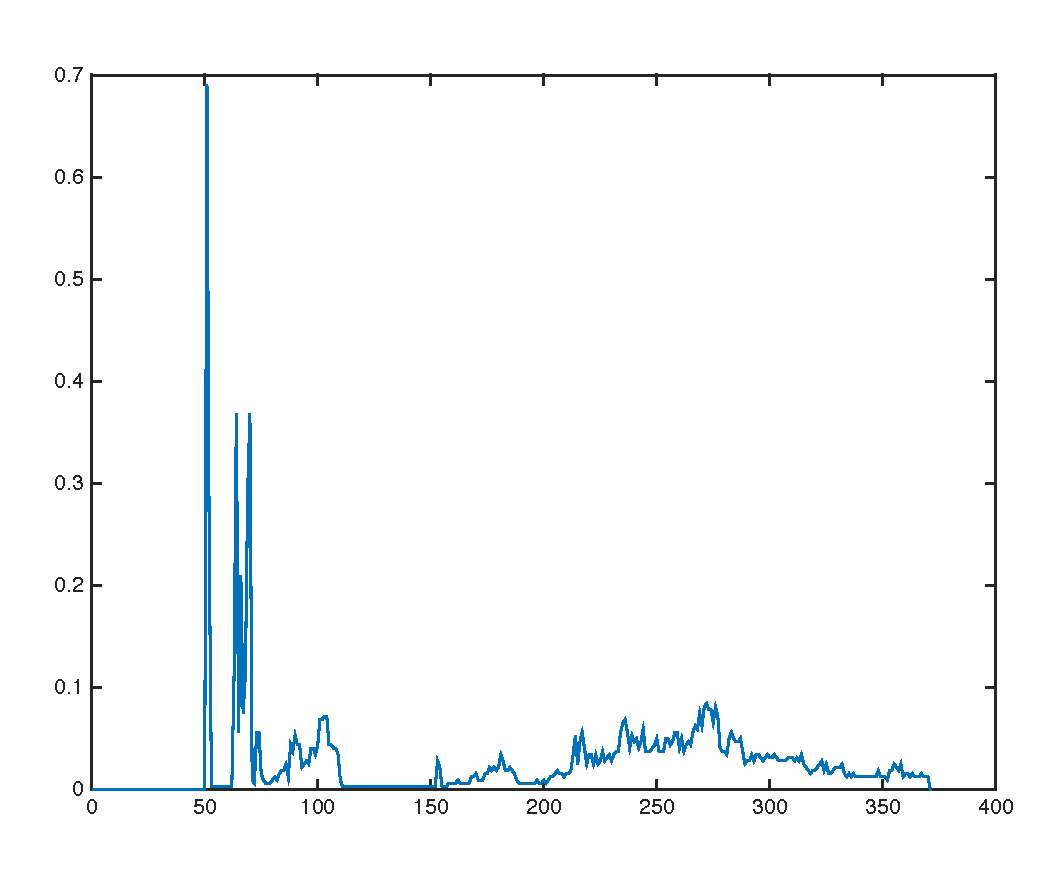
\includegraphics[width=0.8\textwidth]{mean_plot.pdf}
        \captionof{figure}{Example plot of the mean value of the edge image.}
        \label{fig:mean}
    \end{Figure}

    The mean values are then masked against a threshold. The default threshold is \emph{3 * the mean value} of the mean value vector. We then find the last non-zero value of this mask, which gives us the x or y coordinate of the end of the border.

    Since this is done for each layer, the highest value is used. This is because the highest value gives us the border that goes the furthest into our image. The image is then cropped using the found coordinates.

    In order to speed things up a bit, it is assumed that the border has the same width on the left side as it does on the right side, and similarly for the top and bottom.

  \subsection*{Color correction}

    Lastly, the image is color corrected. This is done through gray world assumption. This means that the average intensities of the red and blue channels are normalized to the average intensity of the green channel. The result of this is a RGB image with a gray average intensity.

\section*{Result and discussion}

  The final result of the program can be seen in figure \ref{fig:final_result}.

  While the alignment works well for all tested image, there is a potential problem in the fact that this program does not rotate the images. There might actually be a better match, creating a sharper and more acturate final image, that the program does not find. This is something that could be improved.

  The automatic cropping removes the borders in most cases. However, in some image (mostly those with straight horizontal and vertical lines), the program cannot separate the borders from objects in the photo. Therefore, some photos are cropped more than needed. Fine tuning the threshold used to detect the cropping coordinates could lead to a better result here. As could a more clever method.

  Lastly, the color correction is not perfect for every photo. All it does is to normalize the average intensity, without taking the light source or weather into consideration. This could also be improved.

\end{document}
